\documentclass[11pt,fleqn]{article}
\usepackage[margin=1in]{geometry}
\usepackage{tikz}
\usepackage{mathtools}
\usepackage{longtable}
\usepackage{enumitem}
\usepackage[colorlinks = true,
		linkcolor=black,
		citecolor=black,
	        urlcolor  = black]{hyperref}
%\usepackage[dvips]{graphics}
%\usepackage[table]{xcolor}
%\usepackage{amssymb}
\usepackage{float}
%\usepackage{subfig}
\usepackage{booktabs}
\usepackage{subcaption}
\usepackage{booktabs}

\usepackage[normalem]{ulem}

\usepackage{multicol}
\usepackage{txfonts}
\usepackage{amsfonts}
\usepackage{natbib}

\usepackage{multirow}

\usepackage{gb4e}
\usepackage[all]{xy}
\usepackage{rotating}
\usepackage{tipa}
\usepackage{multirow}
\usepackage{authblk}
\usepackage{url}
\usepackage{pdflscape}
\usepackage{rotating}
\usepackage{adjustbox}
\usepackage{array}

\usepackage{dcolumn} % for printing model output tables directly from R

\usepackage{graphics}
\graphicspath{{../../results/MegaVeridicality/graphs/}}

%\usepackage{color}
%\DeclareOuterCiteDelims{cite}{\textcolor{green}{\bibopenbracket}}{\textcolor{red}{\bibclosebracket}}

\definecolor{Pink}{RGB}{255,50,170}
\newcommand{\jd}[1]{\textcolor{Pink}{[jd: #1]}}  

\newcommand{\jt}[1]{\textbf{\color{purple}JT: #1}}

\newcommand{\tableref}[1]{Tab.~\ref{#1}}
\newcommand{\figref}[1]{Fig.~\ref{#1}}

\def\bad{{\leavevmode\llap{*}}}
\def\marginal{{\leavevmode\llap{?}}}
\def\verymarginal{{\leavevmode\llap{??}}}
\def\swmarginal{{\leavevmode\llap{4}}}
\def\infelic{{\leavevmode\llap{\#}}}

\definecolor{airforceblue}{rgb}{0.36, 0.54, 0.66}
%\definecolor{gray}{rgb}{0.36, 0.54, 0.66}

\newcommand{\dashrule}[1][black]{%
  \color{#1}\rule[\dimexpr.5ex-.2pt]{4pt}{.4pt}\xleaders\hbox{\rule{4pt}{0pt}\rule[\dimexpr.5ex-.2pt]{4pt}{.4pt}}\hfill\kern0pt%
}

\setlength{\parindent}{.3in}
\setlength{\parskip}{0ex}

\newcommand{\yi}{\'{\symbol{16}}}
\newcommand{\nasi}{\~{\symbol{16}}}
\newcommand{\hina}{h\nasi na}
\newcommand{\ina}{\nasi na}

\newcommand{\foc}{$_{\mbox{\small F}}$}

\hyphenation{par-ti-ci-pa-tion}

%\setlength{\bibhang}{0.5in}
%\setlength{\bibsep}{0mm}
%\bibpunct[:]{(}{)}{,}{a}{}{,}

\newcommand{\6}{\mbox{$[\hspace*{-.6mm}[$}} 
\newcommand{\9}{\mbox{$]\hspace*{-.6mm}]$}}
\newcommand{\sem}[2]{\6#1\9$^{#2}$}
\renewcommand{\ni}{\~{\i}}

\newcommand{\citepos}[1]{\citeauthor{#1}'s (\citeyear{#1})}
\newcommand{\citeposs}[1]{\citeauthor{#1}'s}
\newcommand{\citetpos}[1]{\citeauthor{#1}'s \citeyear{#1}}

\newcolumntype{R}[2]{%
    >{\adjustbox{angle=#1,lap=\width-(#2)}\bgroup}%
    l%
    <{\egroup}%
}
\newcommand*\rot{\multicolumn{1}{R{90}{0em}}}% no optional argument here, please!

\title{Hypotheses}

\author{YK and JT}

\begin{document}

\maketitle

\section{Introduction}
We investigate whether and how different parts of the lexical meaning of \emph{that}-clause embedding predicates affect the extent to which the content of the complement clause projects. The basis for our investigation is \citepos{white-rawlins-nels2018} MegaVeridicality dataset, which contains veridicality judgements for 517 predicates. 348 of these predicates were presented to participants in what \cite{white-rawlins-nels2018} refer to as an ``active frame", 142 in  a ``passive frame" and 27 in both. Some predicates in the ``passive frame" are passivised verbal predicates, like \emph{be advised}, others are adjectival predicates, such as \emph{be delighted}. For our investigation, the 27 predicates that occur in both frames are considered separately for each frame, resulting in a total number of 544 predicates.

For their ``measures of veridicality and factivity", \cite{white-rawlins-nels2018} used different sentence frames:
\begin{exe}		
	\ex 
	\begin{xlist}
		\ex Someone \{thought, didn’t think\} that a particular thing happened.
		\ex Someone \{was, wasn’t\} told that a particular thing happened. \hfill(\citealt{white-rawlins-nels2018})
	\end{xlist}
\end{exe}
Following such items, participants were asked, ``Did that thing happen?" (\citealt{white-rawlins-nels2018}). Alternatively, participants saw items in which the question was already included:
\begin{exe}		
	\ex 
	\begin{xlist}
		\ex If someone \{did, didn’t\} know that a particular thing happened, did that thing happen?
		\ex If someone \{was, wasn’t\} told that a particular thing happened, did that thing happen? \\ \null\hfill(\citealt{white-rawlins-nels2018}, slightly modified)
	\end{xlist}
\end{exe}
Projection ratings in the MV dataset are therefore based on three different environments, with the predicates embedded under different (combinations of) entailment-cancelling operators: negation, the antecedent of a conditional and a polar question, or a combination of all three operators. \cite{white-rawlins-nels2018} asked their participants to answer ``yes", ``maybe or maybe not" or ``no". We recoded the corresponding responses as 1, 0 and -1, respectively. 

\section{H1: Predicate type modulates projection}

\subsection{Classification of predicates}
Many of the predicates investigated here can take on different meanings and would have to be categorised differently depending on the specific utterance they are part of. To avoid this potential issue of ambiguity, we classified the predicates strictly based on their meaning in the stimuli used by \cite{white-rawlins-nels2018}. Thus, since the predicates in the MV dataset only occur in the past tense, all of our classifications regarding different parts of their lexical meaning are based solely on their use in the past tense. Similarly, we only considered the meaning of the predicates with the specific ``low lexical content" complement clause used by \cite{white-rawlins-nels2018} for our categorisations.

The main distinction we made for our investigation is that between communicative and private predicates. A predicate \emph{P} is communicative if and only if ``\emph{X} \emph{P}ed that \emph{m}" requires \emph{X} to have externalised that \emph{m} is the case / on the table. This externalisation may be have been verbal or nonverbal. A predicate \emph{P} is private if and only if ``\emph{X} \emph{P}ed that \emph{m}" conveys that \emph{m} stands in some relation to \emph{X}'s mental representation of the world. \emph{X} does not have to believe that \emph{m} is true.

Amongst the private predicates we distinguished between three subtypes: cognitives, emotives and evidentials. A predicate \emph{P} is cognitive if and only if ``\emph{X} \emph{P}ed that \emph{m}" conveys something about \emph{X}'s relation to \emph{m}. A predicate \emph{P} is emotive if and only if ``\emph{X} \emph{P}ed that \emph{m}" conveys that \emph{X} has a feeling or emotion towards \emph{m}. A predicate \emph{P} is evidential if and only if ``\emph{X} \emph{P}ed that \emph{m}" conveys the source of information by which \emph{X} received the information about \emph{m}.

For the small number of predicates which can be used in different ways and would belong to different private predicate types depending on the context, each predicate was assigned to only one private predicate type, depending on which interpretation was considered most likely given \citepos{white-rawlins-nels2018} sentence frame. E.g., \emph{be convinced} can be interpreted as either meaning \emph{be of the conviction} or \emph{be convinced by someone/something}. With the former interpretation, the predicate belongs to the cognitive type; with the latter interpretation, it is an evidential. In this example, the interpretation as a cognitive was considered more likely as it seems more straightforward than assuming an unmentioned source of evidence. 9 predicates that can be used both as communicative and private predicates were excluded from our analysis. 12 predicates we could not assign to any of the predicate types; these were also excluded from analysis. Our results are therefore based on 523 predicates, including 53 cognitives, 236 communicatives, 148 emotives and 86 evidentials.

\subsection{Cognitive vs evidential vs communicative vs emotive predicates}

\figref{projpredtype} shows that the mean projection rating of the emotives in the MV dataset is much higher than that of the other predicate types defined above.

\begin{figure}[H]
	\centering
	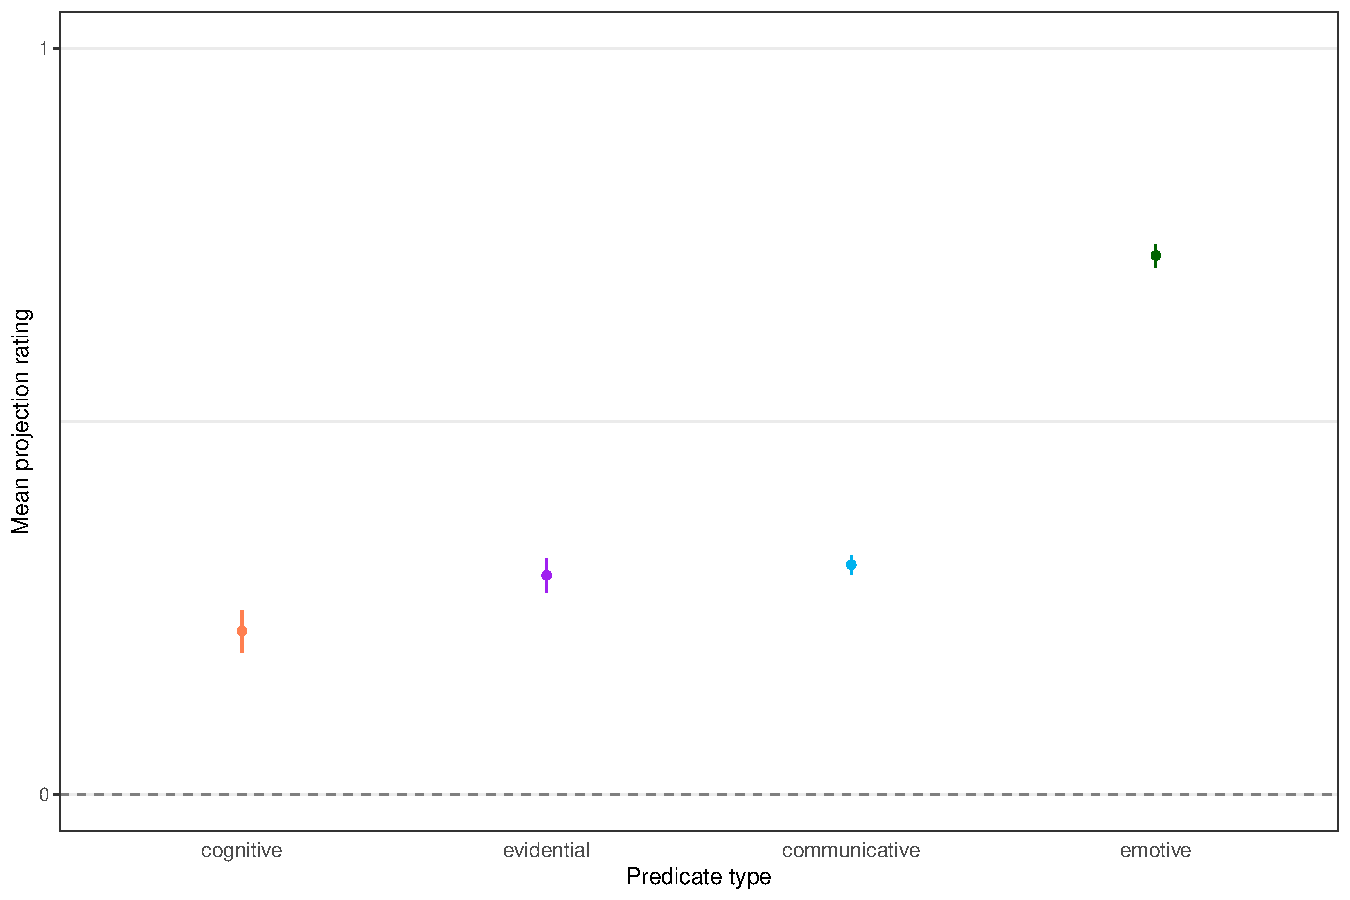
\includegraphics[width=1\textwidth]{projection-by-predicateType}
	\caption{Mean projection rating by predicate type.}
	\label{projpredtype}
\end{figure}

Because the emotives were found to be more projective overall than predicates of the other types, the communicative predicates were subcategorised depending on whether they have an `emotive component' or not. 

\subsection{Communicatives with and without an emotive meaning component}

An emotive meaning component of a communicative is the implication of the emotional state of the speaker that is part of some communicatives, like \emph{sigh} or \emph{snap}, but not others, like \emph{say} or \emph{utter}. Of the 236 communicatives in the MV data set, 47 predicates have an emotive component and 189 do not.

\figref{projpredtype2} shows that the mean projection rating of communicatives with an emotive component, although not nearly as high as for the emotives, is significantly higher than that of the cognitives, evidentials and communicatives without an emotive component. A linear model fitted with the R ``stats" package indicates an effect of each of these five predicate types on the mean projection rating at the 0.001 significance level.

\begin{figure}[H]
	\centering
	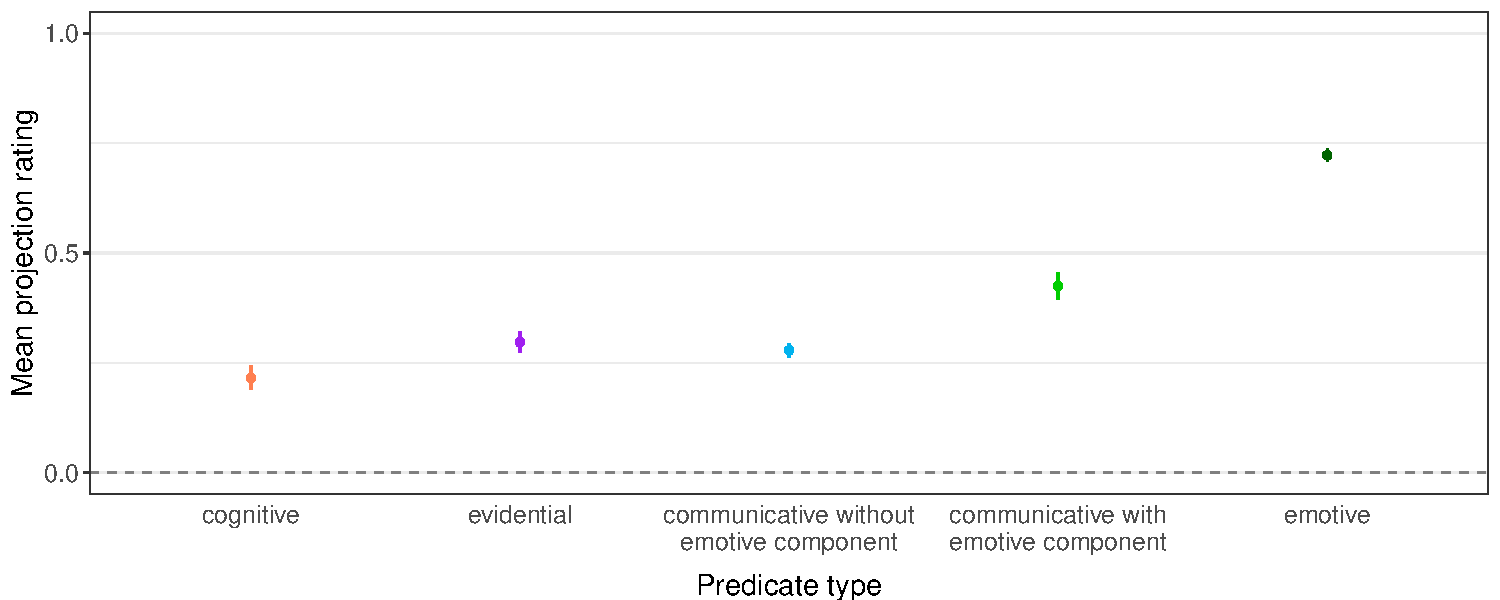
\includegraphics[width=1\textwidth]{projection-by-predicateType2}
	\caption{Mean projection rating by predicate type with distinction between communicatives with and without an emotive meaning component.}
	\label{projpredtype2}
\end{figure}

\figref{projpred} shows again that the emotives have the highest projection ratings overall, followed by the communicates with an emotive meaning component. However, it also highlights high projection variability within each of the predicate types.

\begin{figure}[H]
	\centering
	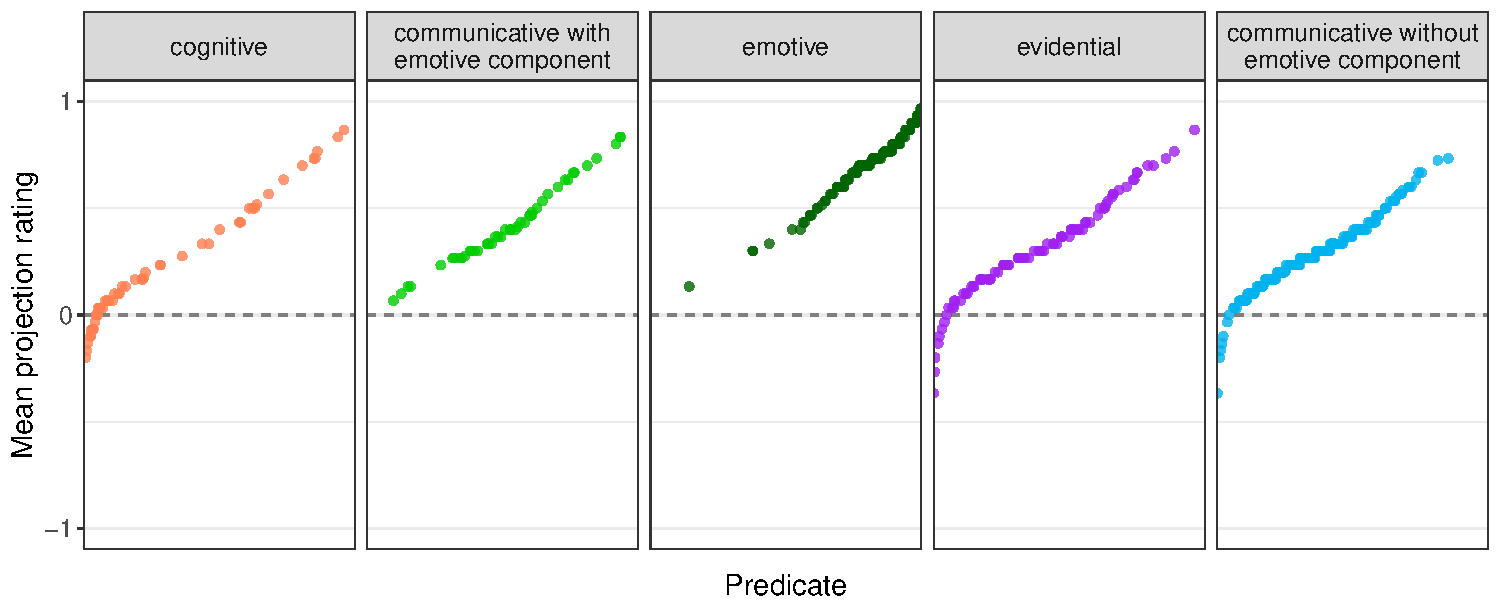
\includegraphics[width=\textwidth]{projection-by-predicate-faceted2}
	\caption{Mean projection rating by predicate and predicate type.}
	\label{projpred}
\end{figure}

Because of the significant differences in projection ratings between the two types of communicatives, this distinction was maintained throughout our investigation.

\subsection{Pure, discourse participation and state changing communicatives}
A further subclassification we made was between `pure', `discourse participation' and `state changing' communicatives. A communicative predicate \emph{P} is pure if and only if \emph{X} can \emph{P} on their own. Conversely, a communicative predicate \emph{P} is a discourse participation communicative if and only if \emph{X} cannot \emph{P} on their own, but the communicative act requires another interlocutor. A communicative predicate \emph{P} is a state changing communicative if and only if \emph{X} cannot \emph{P} on their own and \emph{X}'s communicative act is combined with the intention to change somebody's belief state. We identified 95 pure, 114 discourse participation and 27 state changing communicative predicates in the MV dataset.

\figref{projcomm} shows that the mean projection rating differs significantly between these types of communicatives. A linear model confirms that the effect of each of the three subtypes on the mean projection rating is significant at the 0.001 level.

\begin{figure}[H]
	\centering
	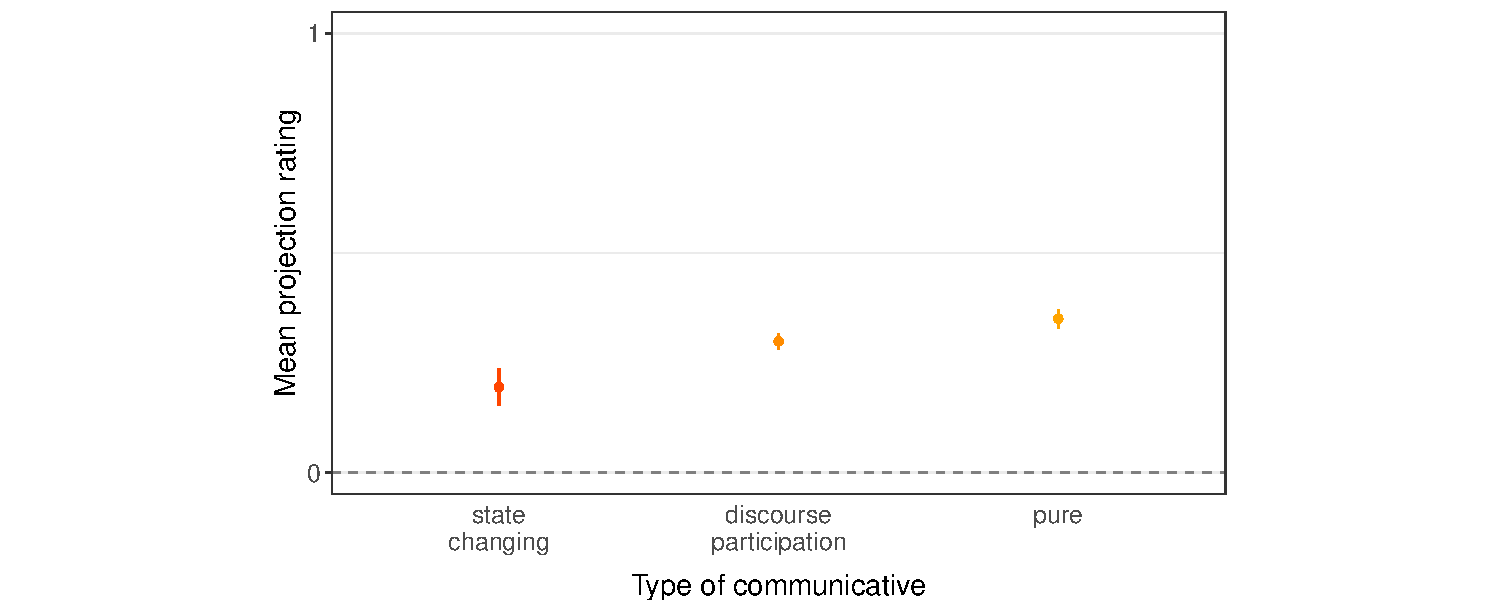
\includegraphics[width=.9\textwidth]{projection-by-predicateType-commType}
	\caption{Mean projection rating by type of communicative.}
	\label{projcomm}
\end{figure}

\figref{projcommfac} comfirms the overall pattern and shows that, as with the main predicate types, there is high by-predicate variability.

\begin{figure}[H]
	\centering
	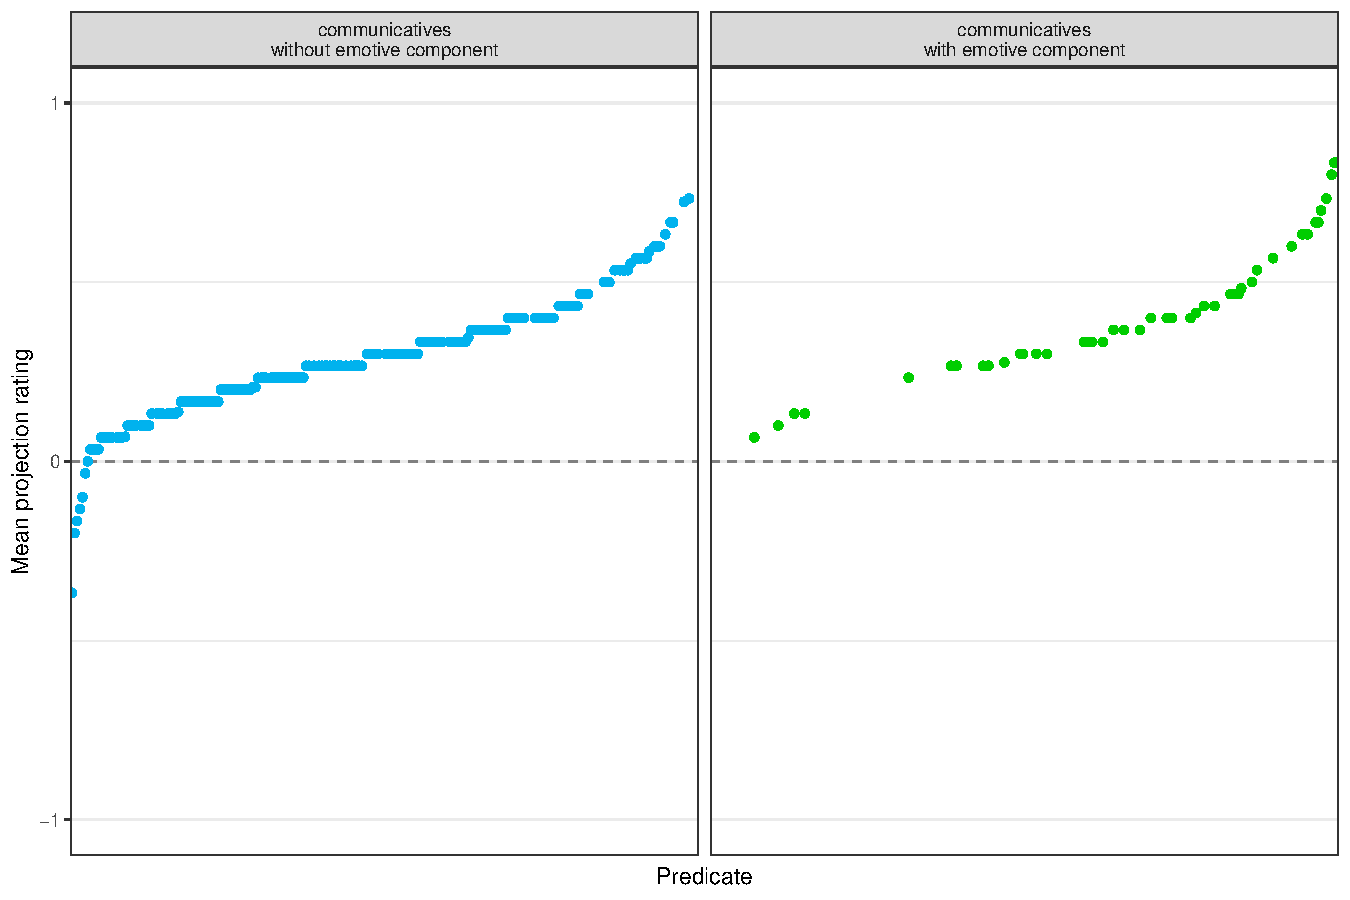
\includegraphics[width=.9\textwidth]{projection-by-communicative-predicate}
	\caption{Mean projection rating by predicate and type of communicative.}
	\label{projcommfac}
\end{figure}


\section{H2: Valence and arousal modulate projection}

The results in sections 2.2 and 2.3 raise the question why the CC of emotive predicates and communicatives with an emotive component projects more than that of other predicates. We therefore investigate whether valence and arousal are the relevant measures of emotivity that predict the projection of the CC.

For this part of our investigation we use \citepos{warriner-etal2013} collection of valence and arousal ratings for 13,915 English lemmas. The dataset contains 428 of the 544 predicates in \citepos{white-rawlins-nels2018} MV dataset: 46 cognitives,  101 emotives, 76 evidentials, 41 communicatives with and 164 communicatives without an emotive component. \citepos{warriner-etal2013} dataset does not contain their raw data, only the mean valence and arousal ratings for each word.

\citepos{warriner-etal2013} participants provided their ratings on scales of 1 to 9, ranging from completely unhappy to completely happy for valence and from completely calm to completely aroused for arousal. The researchers suggest that on both scales, a rating of 5 would indicate a neutral state. However, whilst valence does in fact have a neutral state between the extremes, the neutral state of arousal is not in the middle of the ``calm - aroused" scale, but at its lower end: calmness is the absence of arousal; there is no such thing as `negative' arousal. To make the scales more meaningful for our investigation, they were adjusted in two ways: valence ratings were converted into absolute values of their distance from the neutral state, and the direction of this distance was recorded as an additional variable. Then the ratings for both valence and arousal were rescaled to range from 0 to 1. On this new scale, 0 indicates neutrality and 1 indicates maximum happiness/unhappiness or arousal.

\figref{VAviolins} shows the distribution of valence and arousal ratings within the five predicate types. The ratings for the emotives are most spread out for both valence and arousal. For both variables, the distribution of the ratings for communicatives without an emotive component is quite similar to that of the evidentials. The distribution of valence ratings for the communicatives with an emotive component most closely resembles that of the cognitives, whilst arousal ratings for this predicate type are distributed somewhat similarly to those of the emotives. Overall, this shows that the distribution of valence and arousal ratings correlates with our predicate classifications to some extent. The clear difference in patterns between communicatives with and without an emotive meaning component suggests that we have captured the somewhat vague concept of emotivity quite well, and shows again that we are justified in our decision to consider the two types of communicatives separately.

\begin{figure}[H]
	\centering
	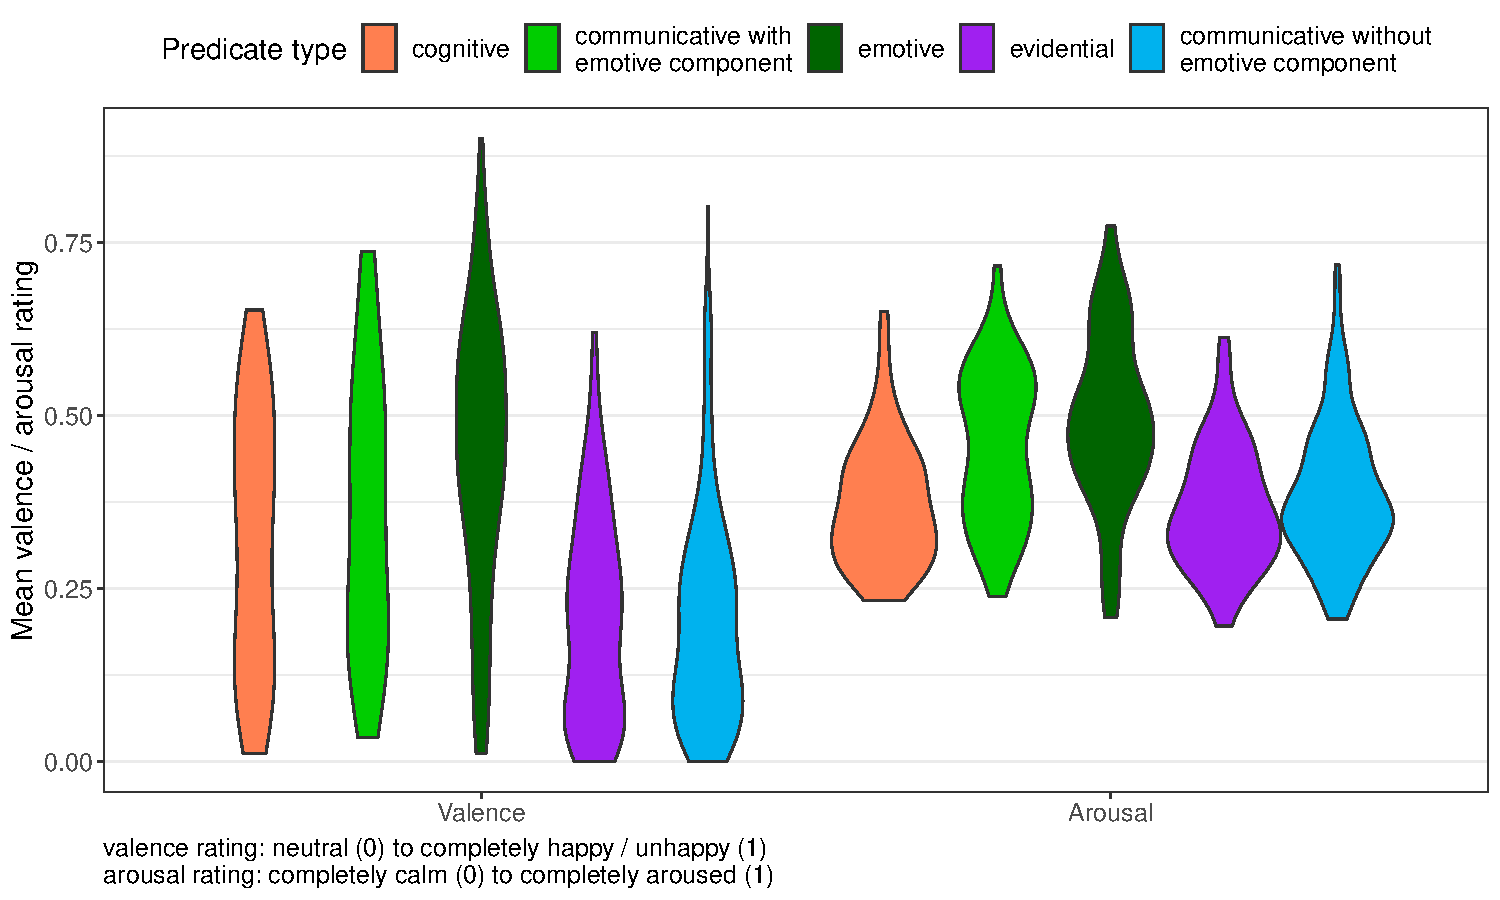
\includegraphics[width=.7\textwidth]{valence-arousal-by-predicateType2}
	\caption{Distribution of mean valence and arousal ratings by predicate type.}
	\label{VAviolins}
\end{figure}

Another similarity between the emotives and the communicatives with an emotive component, in addition to their similarities regarding valence and arousal ratings, is the distribution of the predicates belonging to these types in terms of direction of valence. \tableref{Vdistribution} shows that for these two predicate types, the number of negative valence predicates is much higher than that of positive valence predicates. The opposite is true for the other three predicate types, with a much larger number of positive valence predicates in each of these categories.

\begin{table}[H]
	\centering
	\begin{tabular}{l|c|c} 
		Predicate type & Negative valence & Positive valence \\ 
		\hline
		cognitive & 14 & 32 \\
		communicative with emotive component & 29 & 12 \\
		emotive & 64 & 37 \\
		evidential & 17 & 59 \\
		communicative without emotive component & 61 & 103 \\
	\end{tabular}
	\caption{Distribution of predicates by predicate type and direction of valence.}
	\label{Vdistribution}
\end{table}

These observations raised concerns that our predicate classifications might be so heavily influenced by the factors of valence and arousal that adding predicate type as a variable to our analysis of the patterns discussed below could introduce redundant information and thus obscure the true effects of valence and arousal on projection ratings. If it were indeed the case that our predicate types were based largely on the valence and arousal associated with the predicates assigned to them, then we would expect distinct clusters for each predicate type to emerge in \figref{VAgroups}. Since this is not the case, we conclude that the predicate type variable is sufficiently independent of valence and arousal to justify including both in the same analysis.

\begin{figure}[H]
	\centering
	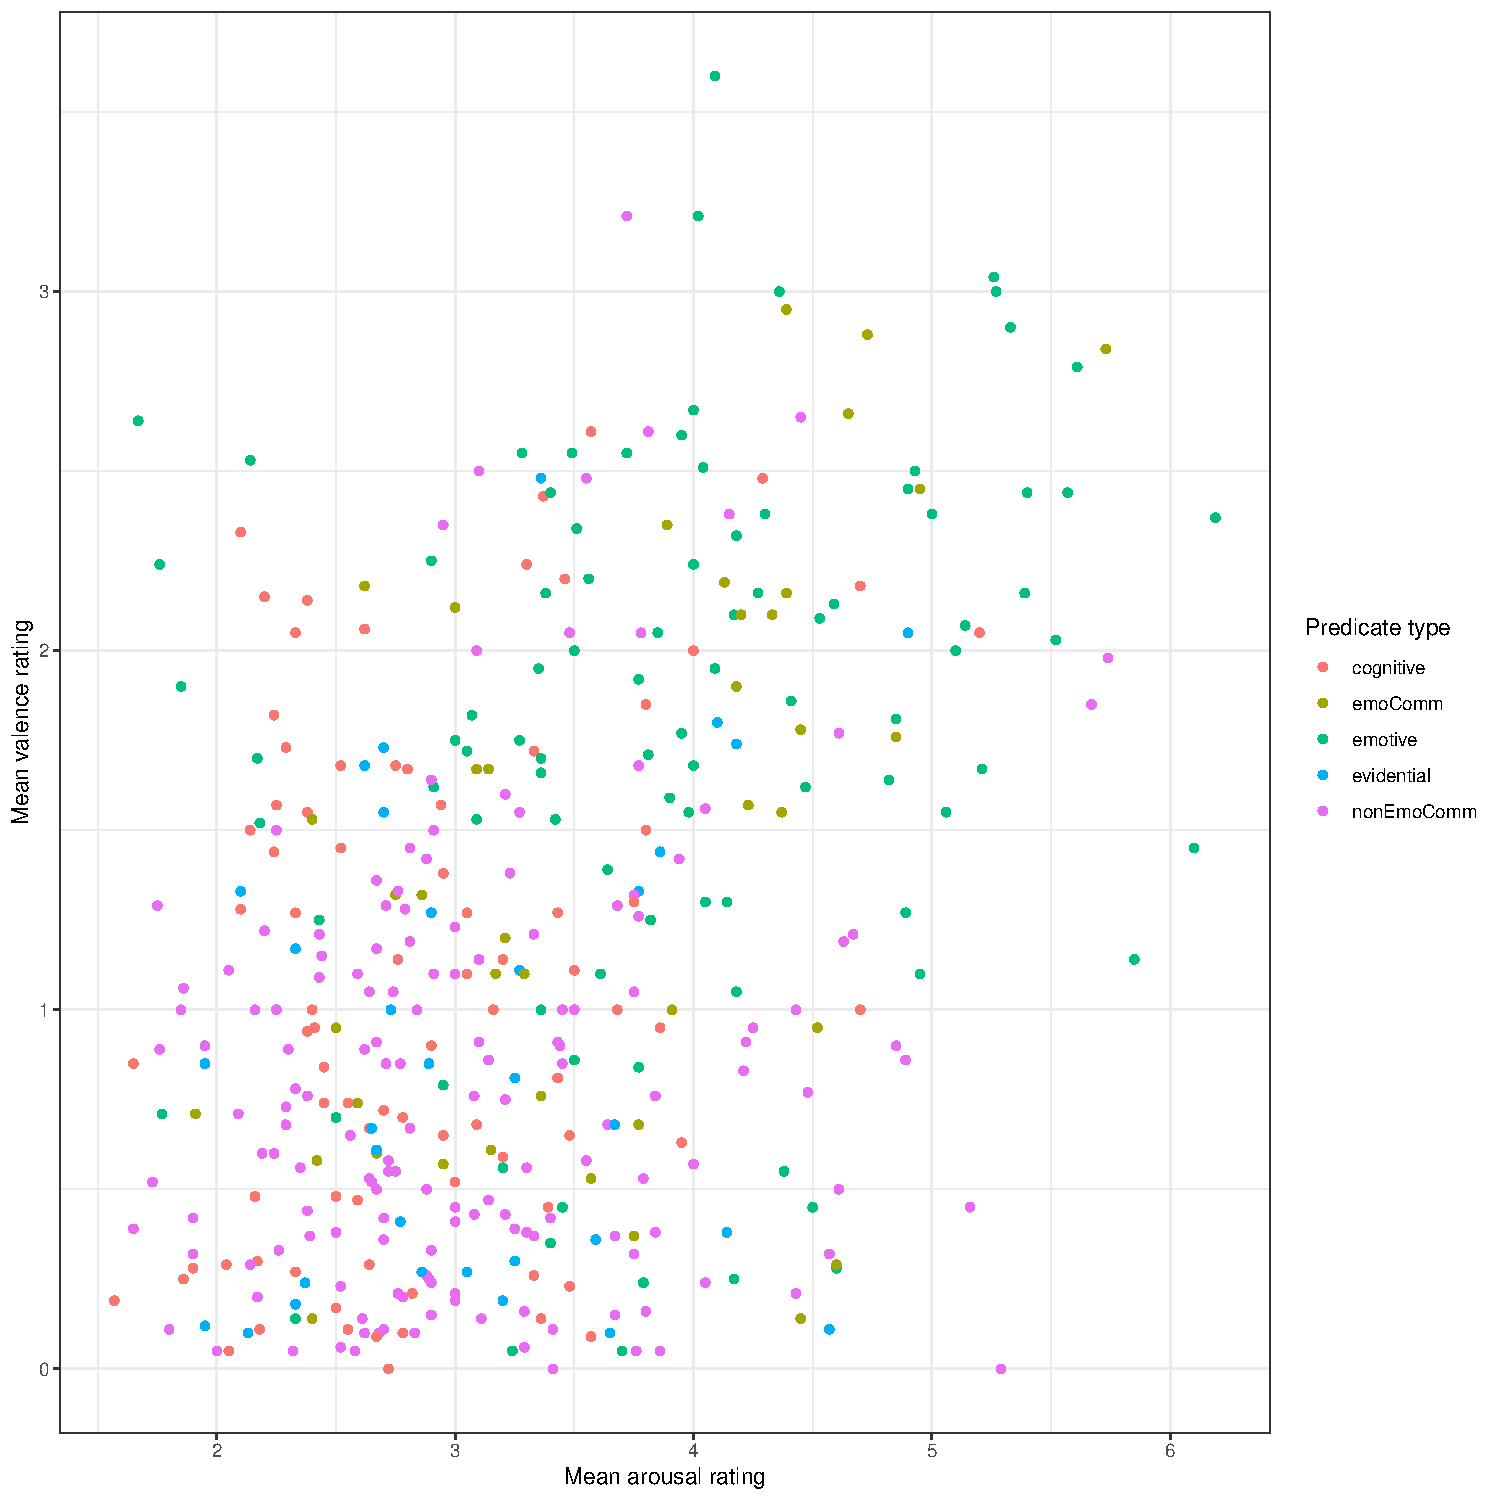
\includegraphics[width=0.65\textwidth]{valence-by-arousal}
	\caption{Mean valence rating by mean arousal rating for 428 predicates grouped by predicate type.}
	\label{VAgroups}
\end{figure}

The effect of valence on projection ratings is shown in \figref{projVdir}. The fitted lines indicate that there is a positive correlation between valence and projection ratings for both negative and positive valence predicates, with the correlation being stronger for negative valence predicates. A cumulative link mixed model fitted with the R package ``ordinal" predicting projection ratings from mean valence ratings and direction of valence with random intercepts for participant and entailment-cancelling environment identifies an effect of valence on projection ratings at the 0.001 significance level.

\begin{figure}[H]
	\centering
	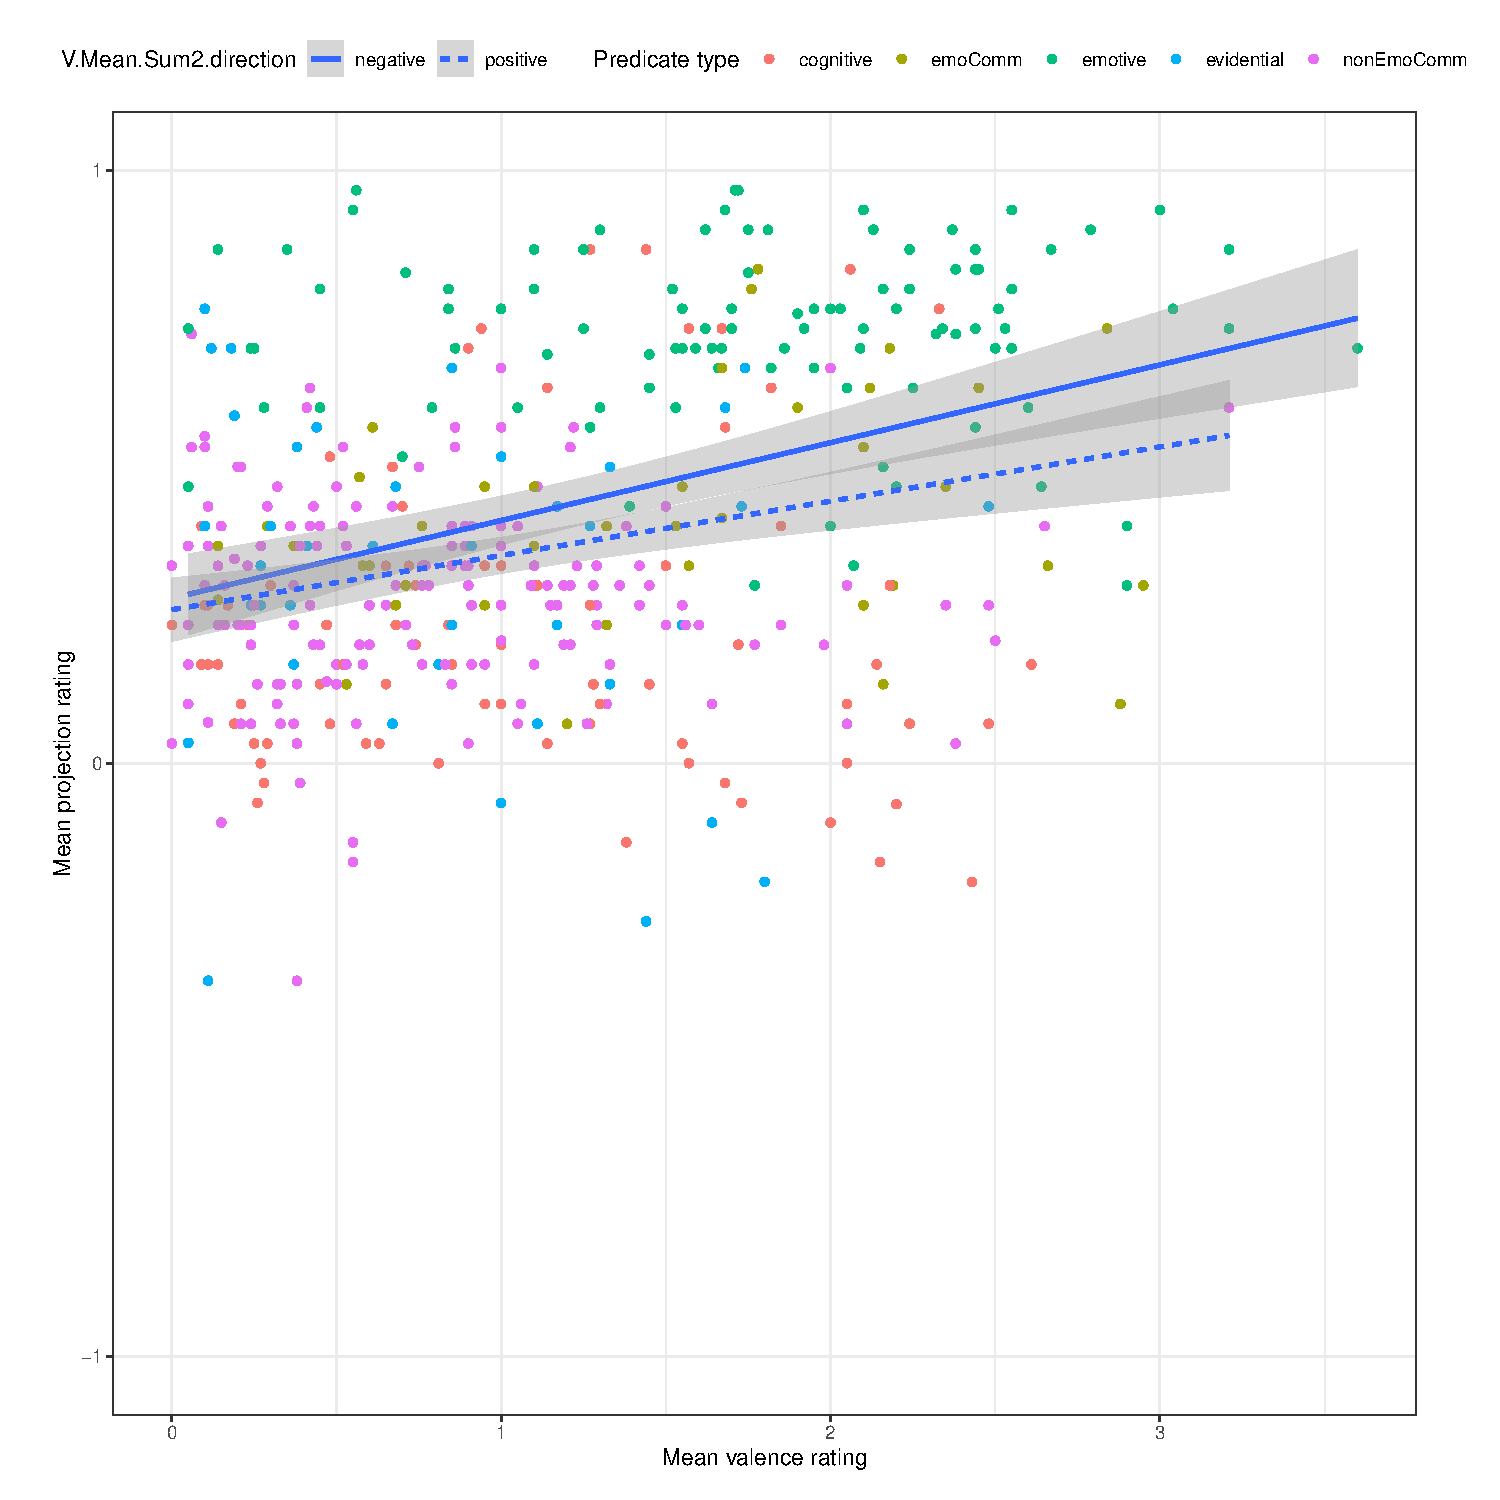
\includegraphics[width=0.65\textwidth]{projection-by-valence-with-direction}
	\caption{Mean projection rating of 428 predicates by mean valence rating and predicate type. Fitted lines show a correlation between valence and projection for predicates with negative and positive valence, respectively.}
	\label{projVdir}
\end{figure}

As \figref{projVfac} shows, this overall pattern no longer holds when the different predicate types are considered separately. The same ordinal model described above with predicate type added as a predictor variable indicates that amongst the predicates with negative valence, valence ratings are only predictive of projection ratings for communicatives with an emotive component; this effect is significant at the 0.001 level. For the predicates with positive valence, the model identifies an effect of valence on projection only for the emotives and the communicatives without an emotive component, both at the 0.05 significance level.

\begin{figure}[H]
	\centering
	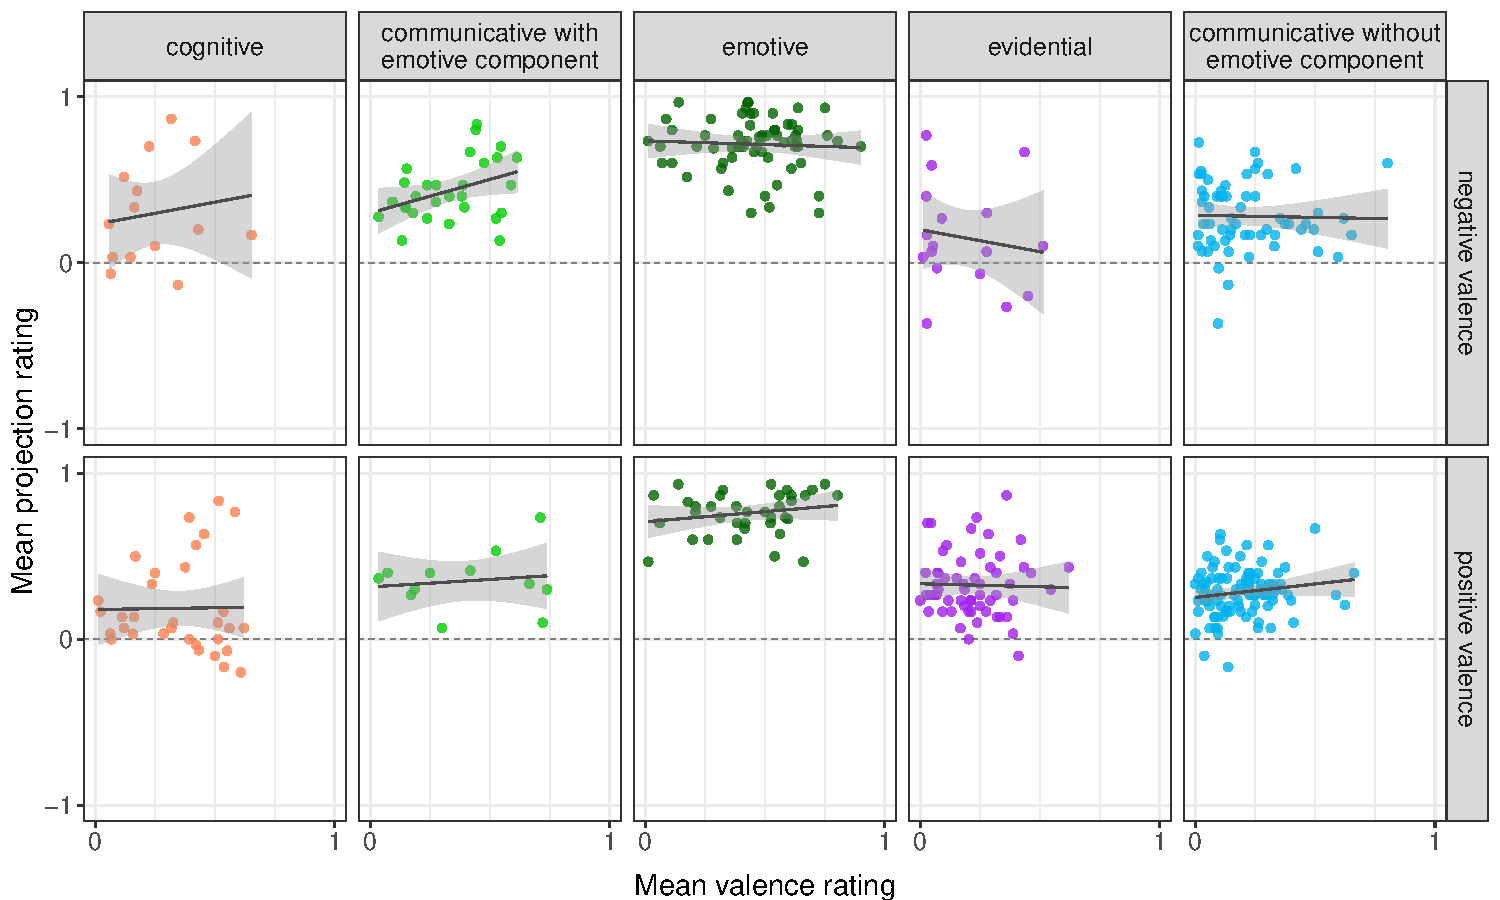
\includegraphics[width=.8\textwidth]{projection-by-valence-and-direction-of-valence-faceted2}
	\caption{Mean projection rating by mean valence rating, predicate type and direction of valence.}
	\label{projVfac}
\end{figure}

\figref{projAdir} shows the effect of arousal on projection ratings. The fitted lines show a positive correlation between arousal and projection ratings for both negative and positive valence predicates. The strength of the correlation appears to be similar for predicates with both valence directions. A cumulative link mixed model predicting projection ratings from mean arousal ratings and direction of valence with random intercepts for participant and environment identifies an effect of arousal on projection ratings at the 0.001 significance level.

\begin{figure}[H]
	\centering
	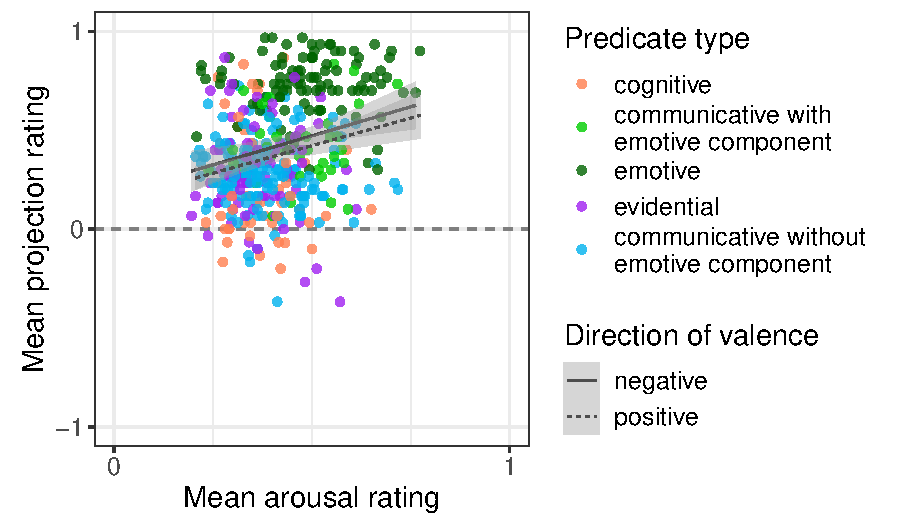
\includegraphics[width=0.65\textwidth]{projection-by-arousal-with-direction}
	\caption{Mean projection rating by mean arousal rating and predicate type for 428 predicates. Fitted lines show the correlation between arousal and projection for predicates with negative and positive valence, respectively.}
	\label{projAdir}
\end{figure}

Like with valence, the overall trend is not found within all predicate types, as shown in \figref{projAfac}. When predicate type is added as a variable to the ordinal model, it identifies arousal rating as predictive of projection rating for the following predicates (with significance level): negative valence emotives (0.05) and communicatives with an emotive component (0.01), positive valence cognitives (0.05), emotives (0.001), communicatives with an emotive component (0.05) and communicatives without an emotive component (0.05).

\begin{figure}[H]
	\centering
	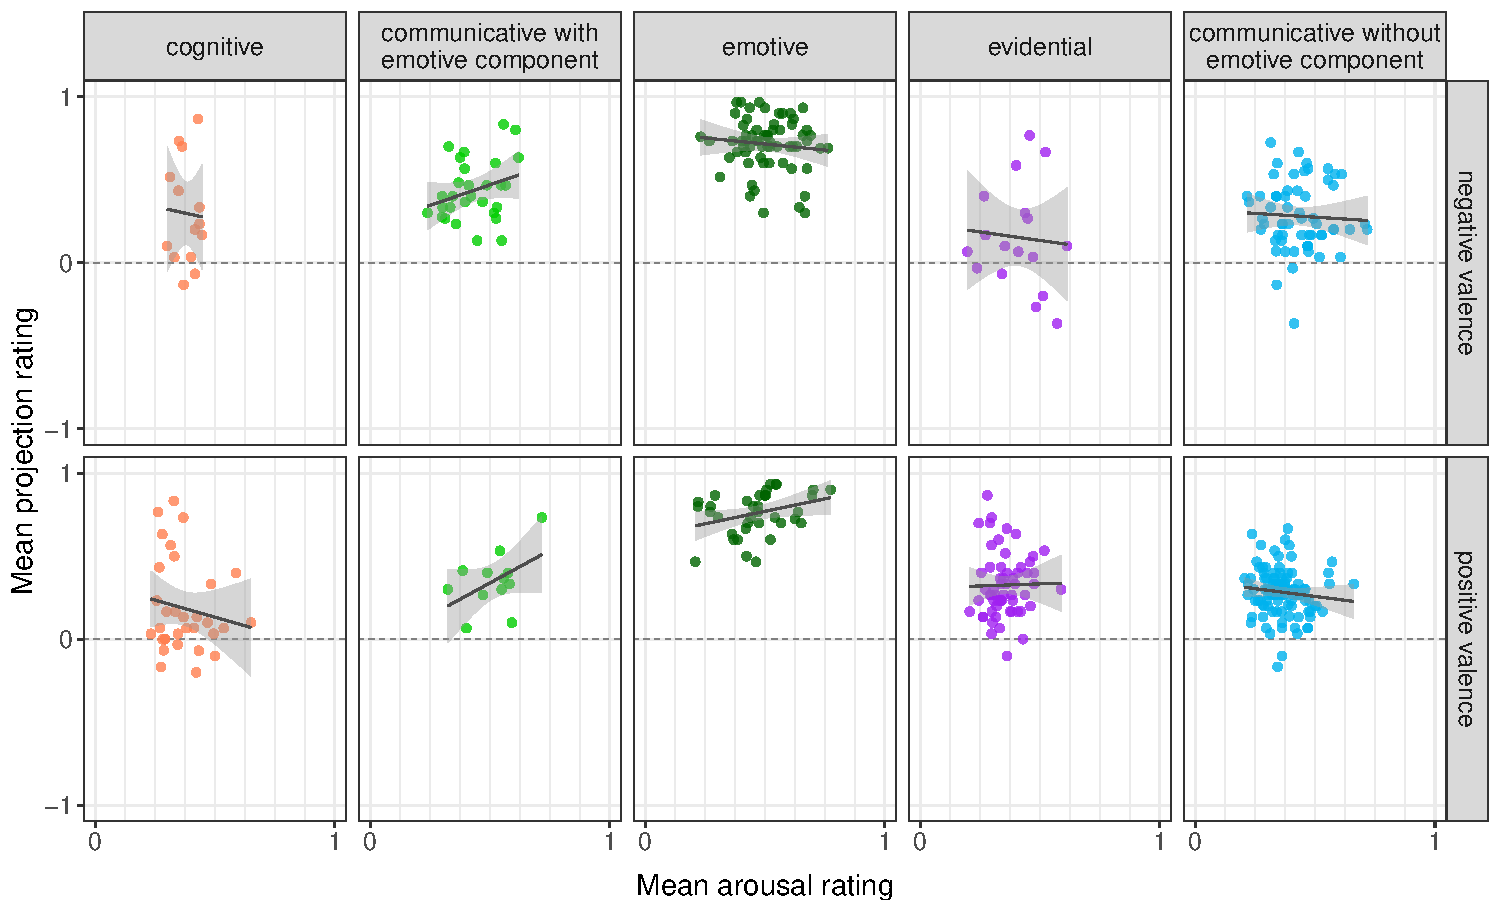
\includegraphics[width=.8\textwidth]{projection-by-arousal-and-direction-of-valence-faceted2}
	\caption{Mean projection rating by mean arousal rating, predicate type and direction of valence.}
	\label{projAfac}
\end{figure}

\section{H3: Dynamicity, change of state and activity modulate projection}

To find out which established distinctions between \emph{that}-clause embedding predicates might matter, we further categorised the predicates as dynamic/stative, non-/change-of-state and non-/activity predicates.

Of the 523 predicates included in our analysis, 39 cognitives, 3 evidentials and all emotives are states. All communicatives are dynamic predicates.

\figref{projdyn} shows that overall, the CC of stative predicates projects more than that of dynamic ones. Within the cognitive and evidential predicate types, however, these differences are not large enough to indicate that the much higher projection ratings of the emotives are entirely the result of their stativity. A linear model indicates an effect of dynamicity on mean projection at the 0.001 significance level. When predicate type is added to the model, dynamicity is no longer significant.

\begin{figure}[H]
	\centering
	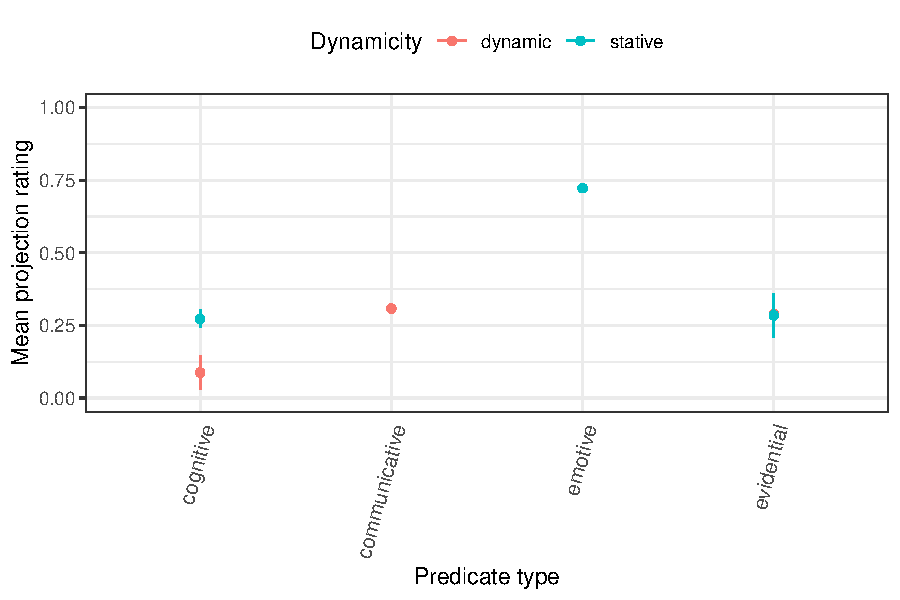
\includegraphics[width=1\textwidth]{projection-by-predicateType-and-Dynamicity}
	\caption{Mean projection rating by predicate type and dynamicity.}
	\label{projdyn}
\end{figure}

Change-of-state predicates were identified based on whether the predicate denotes a change in the attitude holder from a state of unawareness/uncertainty/undecidedness to a state of awareness/certainty/decidedness. There are 40 change-of-state predicates amongst those whose projection ratings we analysed: 2 cognitives and 38 evidentials.

\figref{projcos} shows a much higher mean projection rating for change-of-state cognitives than for their non-change-of-state counterparts. However, as this mean is based on only two predicates, the difference cannot be considered indicative of a general pattern. Amongst the evidentials, whether a predicate denotes a change of state or not does not seem to affect projection. A linear model shows an overall effect of the change-of-state status of a predicate on projection at the 0.001 significance level. With predicate type as an additional variable, the model confirms that the difference between mean projection ratings of the two subgroups of evidentials is not significant.

\begin{figure}[H]
	\centering
	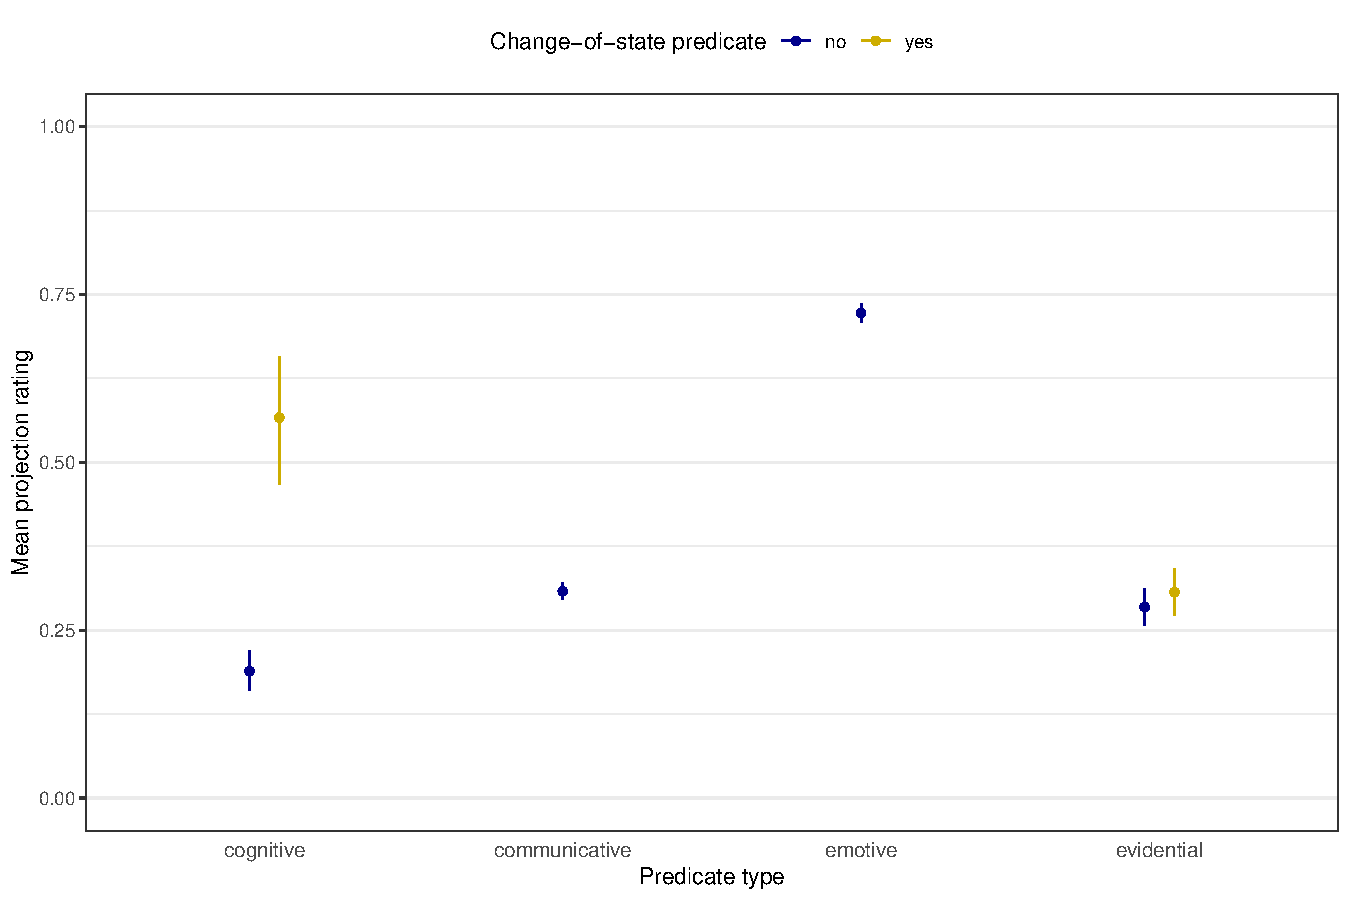
\includegraphics[width=1\textwidth]{projection-by-predicateType-and-CoS}
	\caption{Mean projection rating by predicate type and non-/change-of-state predicate distinction.}
	\label{projcos}
\end{figure}

Of the 523 predicates considered here, 12 cognitives, 44 communicatives with an emotive component, 12 evidentials and 95 communicatives without an emotive component were classified as activities. All emotives are states.
\figref{projact} does not show a clear pattern. Amongst the cognitives, the mean projection rating of those predicates that are not an activity is significantly higher than that of the activities. The non-activity communicatives with an emotive component have a slightly higher mean projection rating than the activities in this predicate type. The evidentials show the opposite pattern. Amongst the communicatives without an emotive component, there appears to be no significant difference between the mean projection ratings of non-/activity predicates. A linear model shows that overall, there is an effect of activity on projection at the 0.001 significance level. For the individual predicate types, the effect is only significant for the cognitives, where it is at the 0.001 significance level.

\begin{figure}[H]
	\centering
	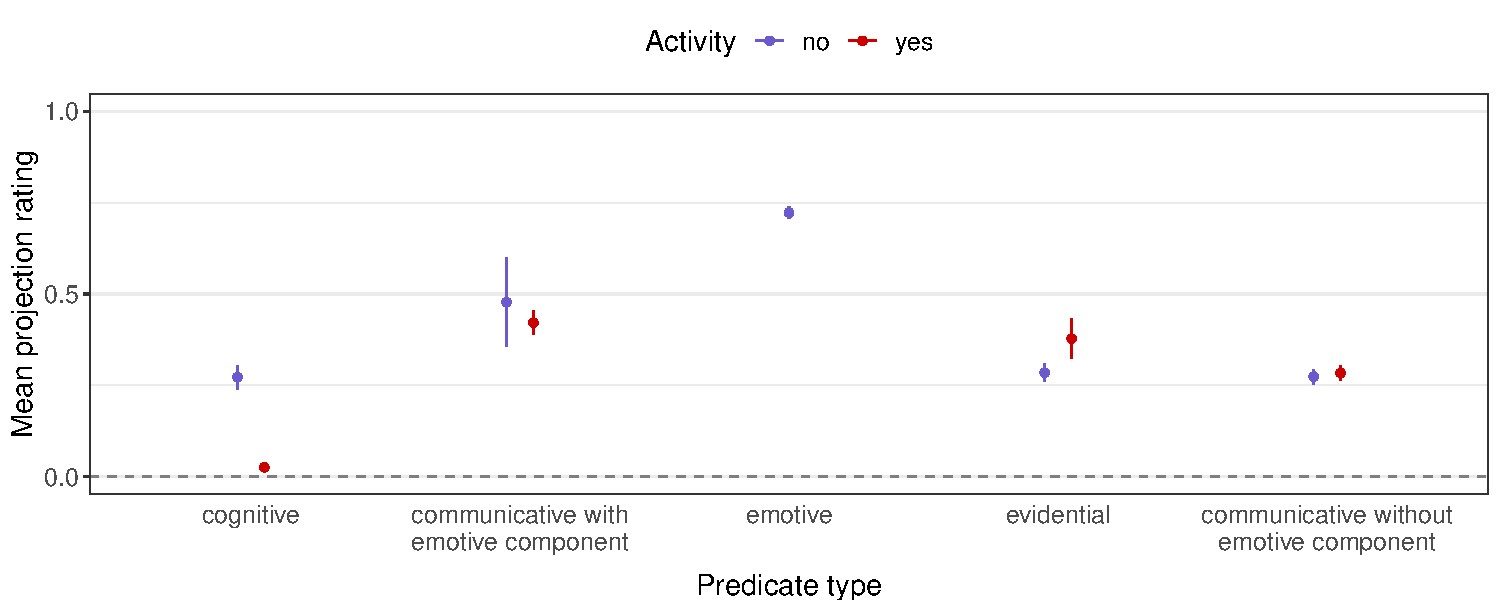
\includegraphics[width=1\textwidth]{projection-by-predicateType-and-activity}
	\caption{Mean projection rating by predicate type and non-/activity distinction.}
	\label{projact}
\end{figure}

In \figref{projcomb}, the different features of predicate meaning discussed above are shown side by side for easier comparison. The plot highlights that neither of the investigated categories can be considered predictive of projection across all predicate types. Patterns that seem to emerge within predicate types are largely due to the uneven distribution of activities, change-of-state predicates and states.

\begin{figure}[H]
	\centering
	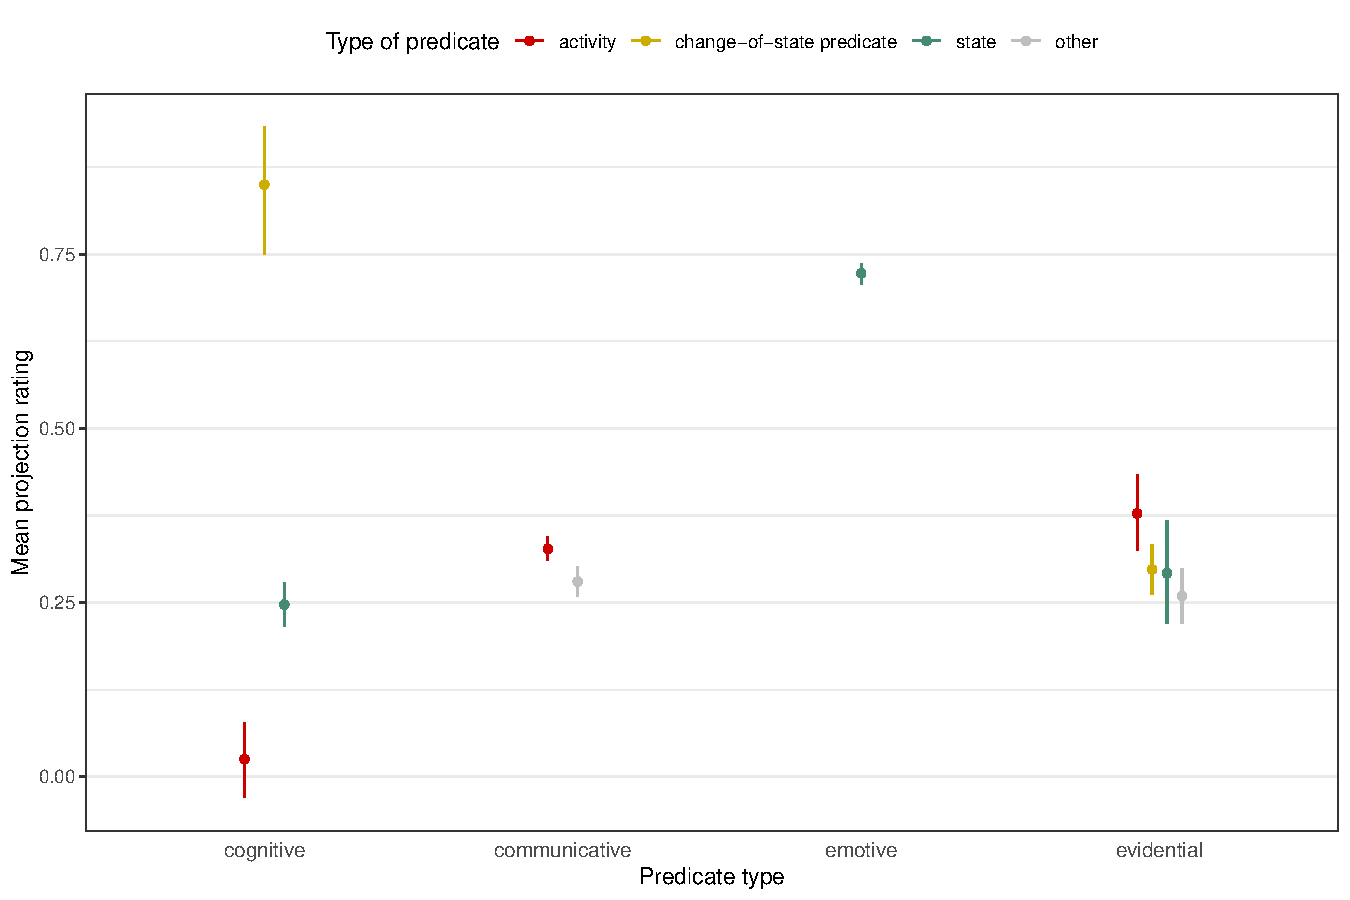
\includegraphics[width=1\textwidth]{projection-by-predicateType-and-stateActivityCoS}
	\caption{Mean projection rating by predicate type and activity / change of state / stativity.}
	\label{projcomb}
\end{figure}

\tableref{acossdistribution} shows the distribution of the different kinds of predicates for each of our predicate types. It highlights that in all predicate types, certain kinds of predicates occur very rarely or not at all. This seems to suggest that factors related to activity, dynamicity and change-of-state properties are already reflected to some extent in our predicate types, similar to how factors related to valence and arousal are part of, but do not define, the nature of our predicate types, as discussed in section 3.

\begin{table}[H]
	\centering
	\begin{tabular}{l|c|c|c|c} 
		Predicate Type & Activity & CoS predicate & State & Other \\ 
		\hline
		cognitive & 12 & 2 & 39 & -- \\
		communicative with emotive component & 44 & -- & -- & 3 \\
		emotive & -- & -- & 148 & -- \\
		evidential & 12 & 38 & 3 & 33 \\
		communicative without emotive component & 95 & -- & -- & 94 \\
	\end{tabular}
	\caption{Distribution of predicates by predicate type and activity / change of state / state / other.}
	\label{acossdistribution}
\end{table}

\figref{projcombfac} shows again that overall, the CC of stative predicates projects more strongly than that of activities, change-of-state predicates or others. It furthermore shows high projection variability within each of these categories.

\begin{figure}[H]
	\centering
	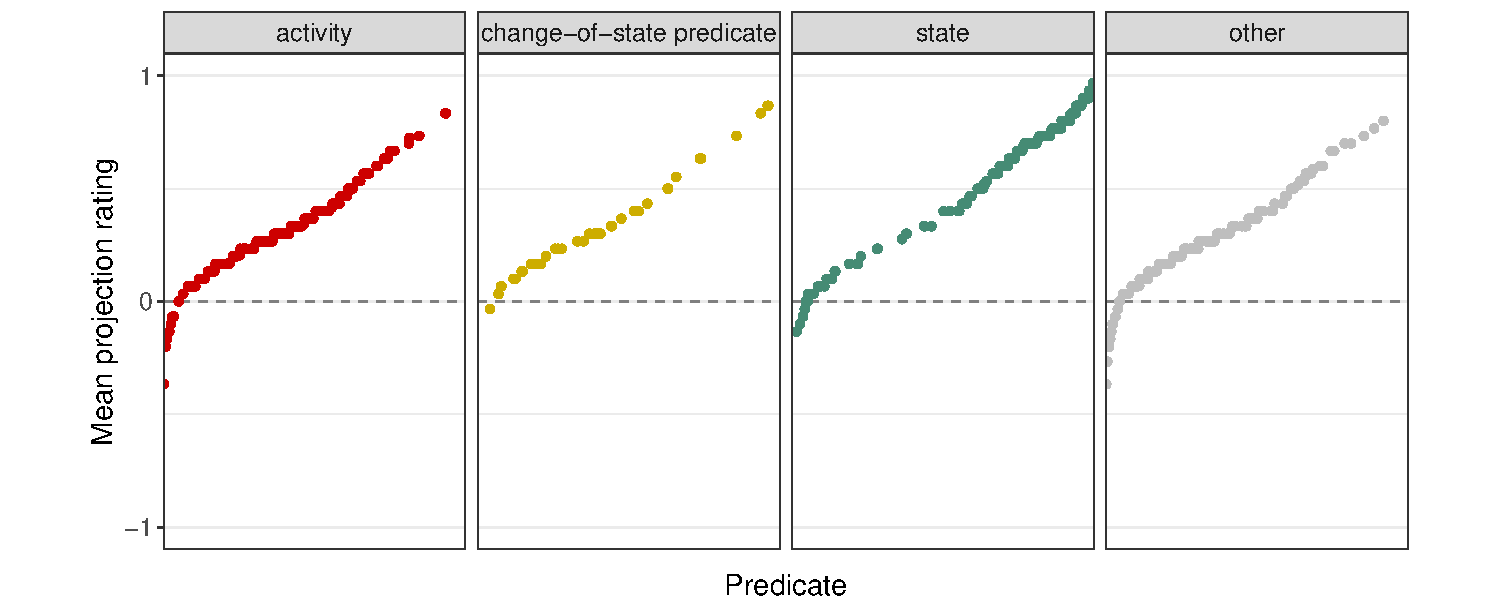
\includegraphics[width=.8\textwidth]{projection-by-predicate-stateActivityCoS-faceted}
	\caption{Mean projection rating by predicate and activity / change of state / stativity / other.}
	\label{projcombfac}
\end{figure}


\section{H4: Positive correlation between veridicality and projection ratings}
Another category we have to include in our investigation of factors that might affect projection is that of ``factive predicates", whose CC is presupposed and therefore expected to project (\citealt{kiparsky-kiparsky70}). As it has been claimed that the CC of these predicates is not only presupposed but also entailed (e.g., \citealt{anand-hacquard2014}), we investigate the correlation between veridicality and projection ratings in \citepos{white-rawlins-nels2018} MV dataset. The responses we consider `veridicality ratings' are those based on the affirmative sentence frame in the dataset.

\figref{projverid} shows a positive correlation between veridicality and projection ratings for all predicate types. A cumulative link mixed model predicting projection ratings from mean veridicality ratings with random intercepts for participant and environment shows that the overall effect is significant at the 0.001 level. The effect is significant at the same level for each of the predicate types. We used mean veridicality ratings rather than the individual ratings as our predictor variable because of how the data were collected: most of \citepos{white-rawlins-nels2018} participants only completed one list, each of which contained 68 different predicates in only one sentence frame, i.e., participants did not provide projection and veridicality ratings for the same predicates.

\begin{figure}[H] 
	\centering
	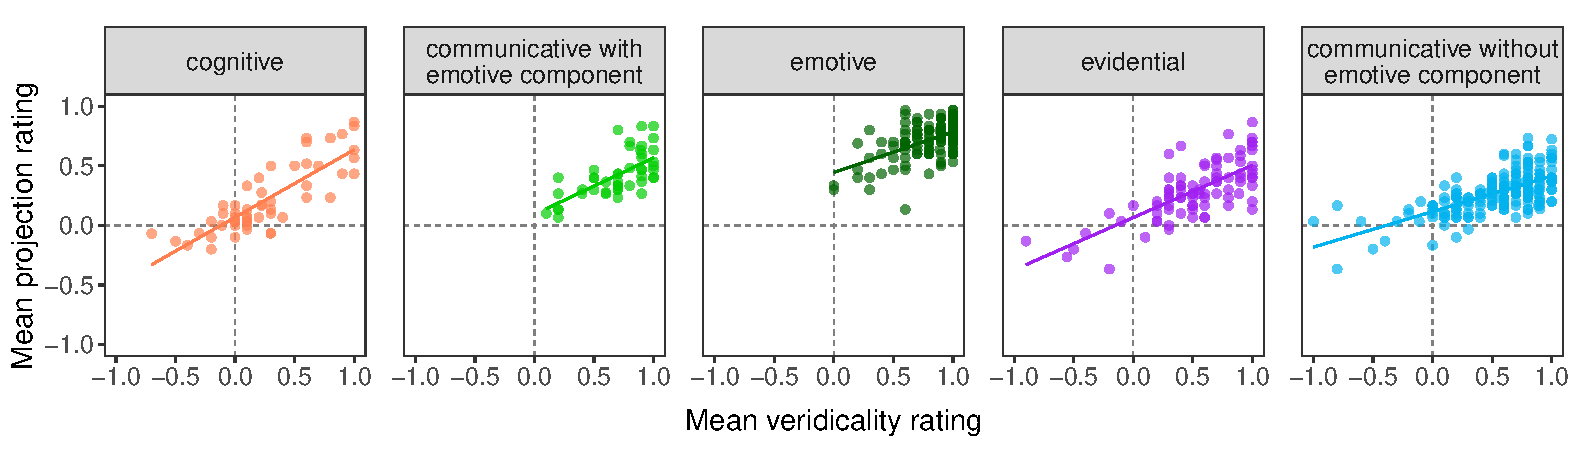
\includegraphics[width=.9\textwidth]{projection-by-veridicality2-faceted}
	\caption{Mean projection rating by mean veridicality rating and predicate type.}
	\label{projverid}
\end{figure}

\figref{projveridfactives} shows the positive correlation between veridicality and projection ratings for all predicates. It further shows that all canonically projective predicates in the MV dataset are located in the upper right quadrant of the plot and that for most of these predicates, both veridicality and projection ratings are relatively high.

\begin{figure}[H] 
	\centering
	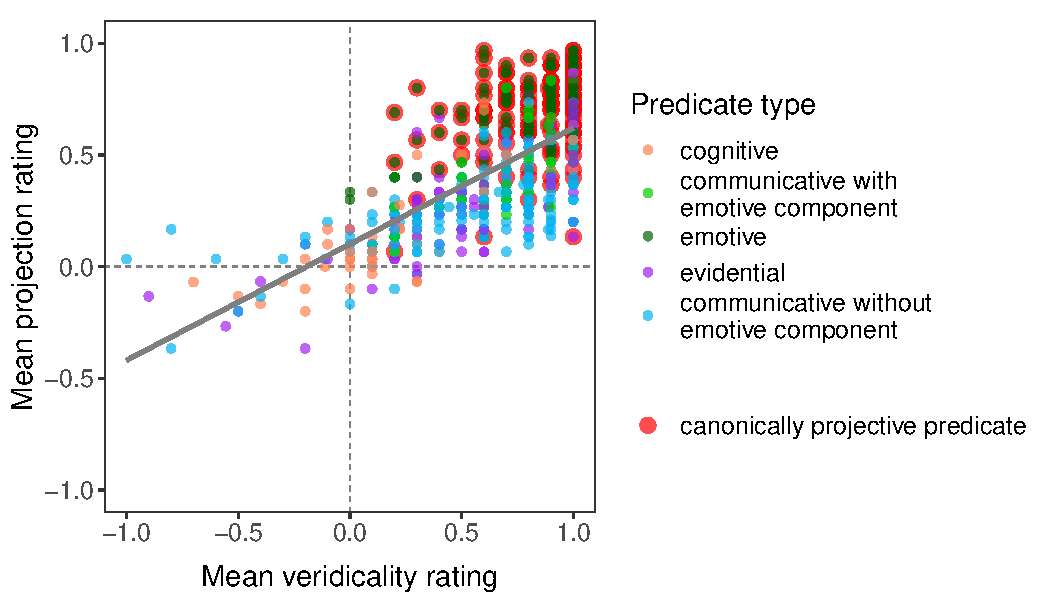
\includegraphics[width=0.6\textwidth]{projection-by-veridicality-with-factives2}
	\caption{Mean projection rating by mean veridicality rating and predicate type for 523 predicates with canonically projective predicates highlighted.}
	\label{projveridfactives}
\end{figure}



\section{H5: Interaction of environment with predicate type}

As described in section 1, the projection ratings collected by \cite{white-rawlins-nels2018} are based on predicates occurring in different entailment-cancelling environments. Since \cite{hofmann-etal23} showed an effect of different entailment-cancelling environments on projection and raised the question how this might interact with the meaning of the predicates, we examine the interaction of this factor with our predicate types. 

As shown in \figref{projpredtypeenv}, there are significant differences between the mean projection ratings for the three types of environments within all predicate types except the cognitives. The other four predicate types also show the same pattern in terms of projection strength, with the lowest mean projection ratings for items with all three entailment-cancelling operators, significantly higher ratings for items with negation only, and again significantly higher ratings for question and conditional items.

\begin{figure}[H]
	\centering
	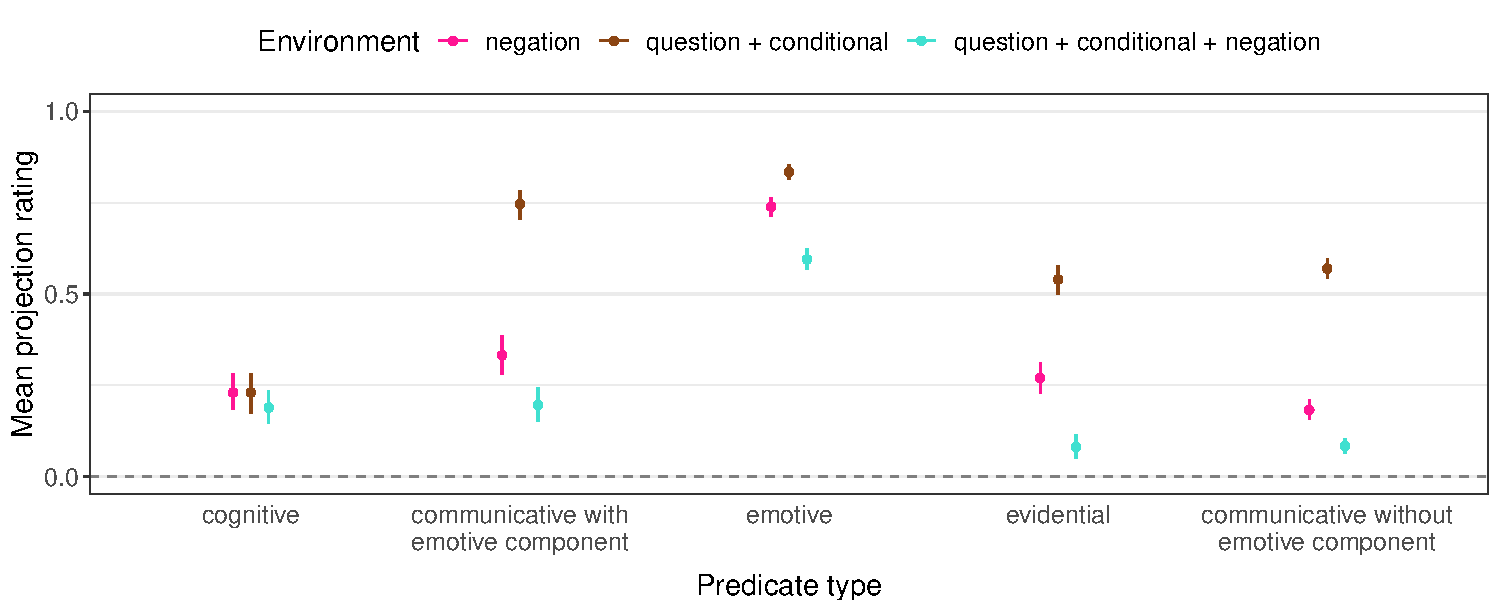
\includegraphics[width=1\textwidth]{projection-by-predicateType-and-environment}
	\caption{Mean projection rating by predicate type and entailment-cancelling environment.}
	\label{projpredtypeenv}
\end{figure}

\figref{projpredtypeenvfac} shows the mean projection rating by predicate for all combinations of entailment-cancelling environment and predicate type. It highlights again the overall higher projection ratings based on the question and conditional environment compared to the other two environments. The plot further shows again that the cognitives behave differently, especially in the question and conditional environment. Moreover, the figure shows that there is high projection variability in all environment--predicate type combinations.

\begin{figure}[H]
	\centering
	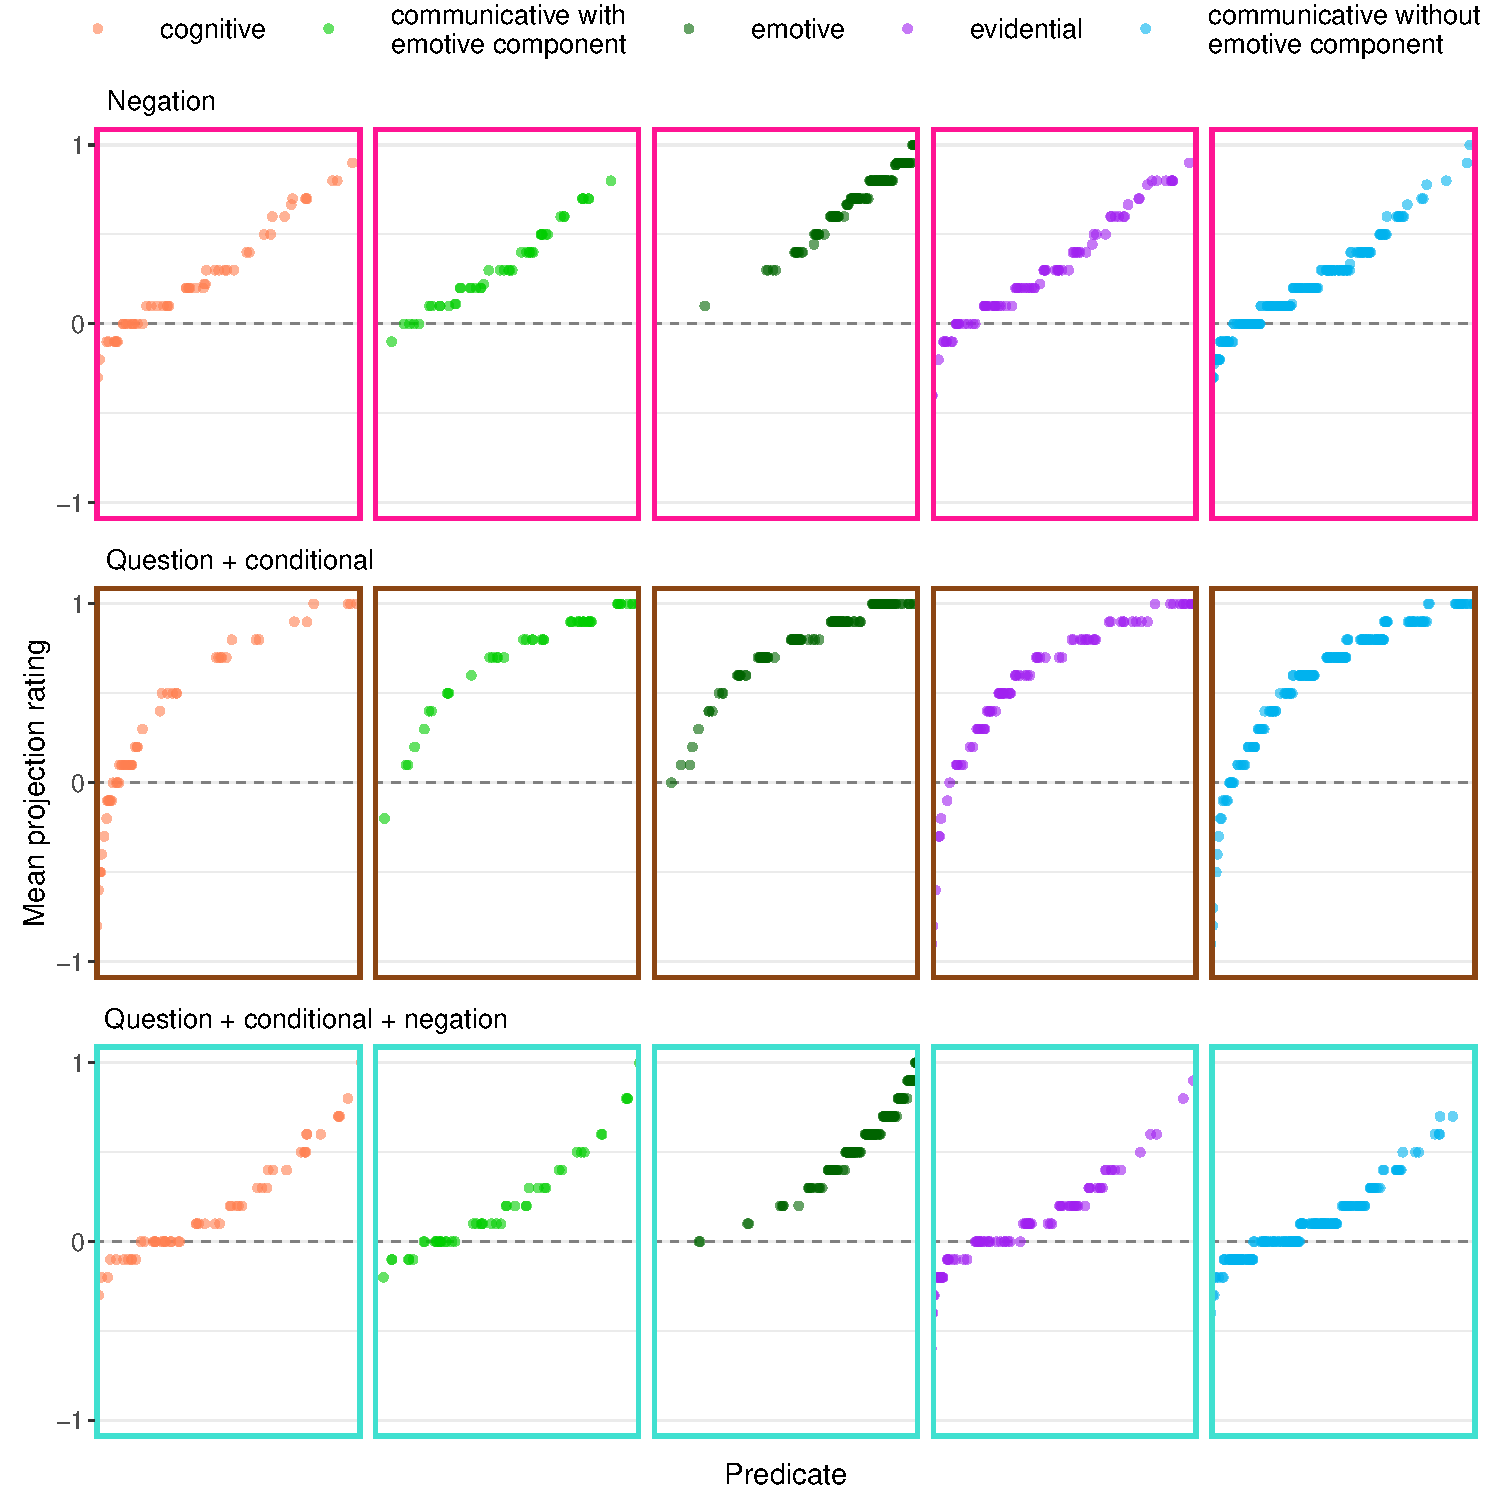
\includegraphics[width=0.9\textwidth]{projection-by-predicateType-and-environment-faceted}
	\caption{Mean projection rating by predicate, environment and predicate type.}
	\label{projpredtypeenvfac}
\end{figure}

\section{Conclusion}
We have shown that projection ratings in the MV dataset are influenced by several factors. Most of these are less significant or no longer significant at all once predicate type is added as a variable. The exception to this is veridicality, which is a strong predictor of projection regardless of predicate type. Predicate type itself strongly predicts projection ratings. Our results show that the five predicate types we have assumed for our investigation are clearly distinguishable, even with regard to factors that we did not deliberately include in their definitions. These factors, or aspects related to them, can therefore be expected to affect projection ratings via predicate type. In order to take this into account in statistical analyses, we should examine our predicate types in more detail and describe the patterns they show regarding the factors investigated here. In addition, we should look into what kind of ordinal model we can use to produce interpretable results on the effects of only categorical variables, in order to provide more solid evidence for our findings.


\bibliographystyle{../cslipubs-natbib}
\bibliography{../bibliography}


\end{document}
